\documentclass[11pt,a4paper]{article}
\usepackage[T1]{fontenc}
\usepackage[spanish]{babel}
\usepackage[margin=22mm]{geometry}
\usepackage{mathptmx,graphicx,tabularx,booktabs,xcolor}
\usepackage[hidelinks]{hyperref}
\setlength{\parindent}{0pt}
\setlength{\parskip}{.5em}
\definecolor{Pendiente}{HTML}{B3261E}
\newcommand{\campo}[1]{\textcolor{Pendiente}{[#1]}}
% Reparto acordado. Cada integrante completa su proyecto.
\newcommand{\personaUno}{Belinda Toaquiza}
\newcommand{\personaDos}{Allison Mera}
\newcommand{\personaTres}{Eduardo Reinoso}
\newcommand{\personaCuatro}{Byron Daniel Loor}
\newcommand{\proyectoUno}{\campo{Proyecto 1}}
\newcommand{\proyectoDos}{\campo{Proyecto 2}}
\newcommand{\proyectoTres}{\campo{Proyecto 3}}
\newcommand{\proyectoCuatro}{\campo{Proyecto 4}}

\newcommand{\espacio}{\par\rule{\linewidth}{.3pt}\par\vspace{5mm}}
\begin{document}
% Notas del integrante 1. Compilar notas/main.tex.
\section*{\personaUno · RPC}
\textbf{Proyecto}\quad \proyectoUno
\subsection*{Teoría y ejemplo sencillo}
\campo{Escribir lo que se dirá sobre RPC, el contrato, la entrada y la salida de la demo.}
\espacio
\subsection*{Aplicación futura al proyecto}
\campo{Explicar el estado actual y qué servicio se implementaría. Añadir la operación, motivación, transparencias, CAP/PACELC y comparación con fuentes.}
\espacio
\subsection*{Fallo supuesto y conclusión}
\campo{Describir causa, impacto, detección, recuperación propuesta y prueba de validación.}
\espacio
\textbf{Bosquejo a mano}\quad
\begin{center}
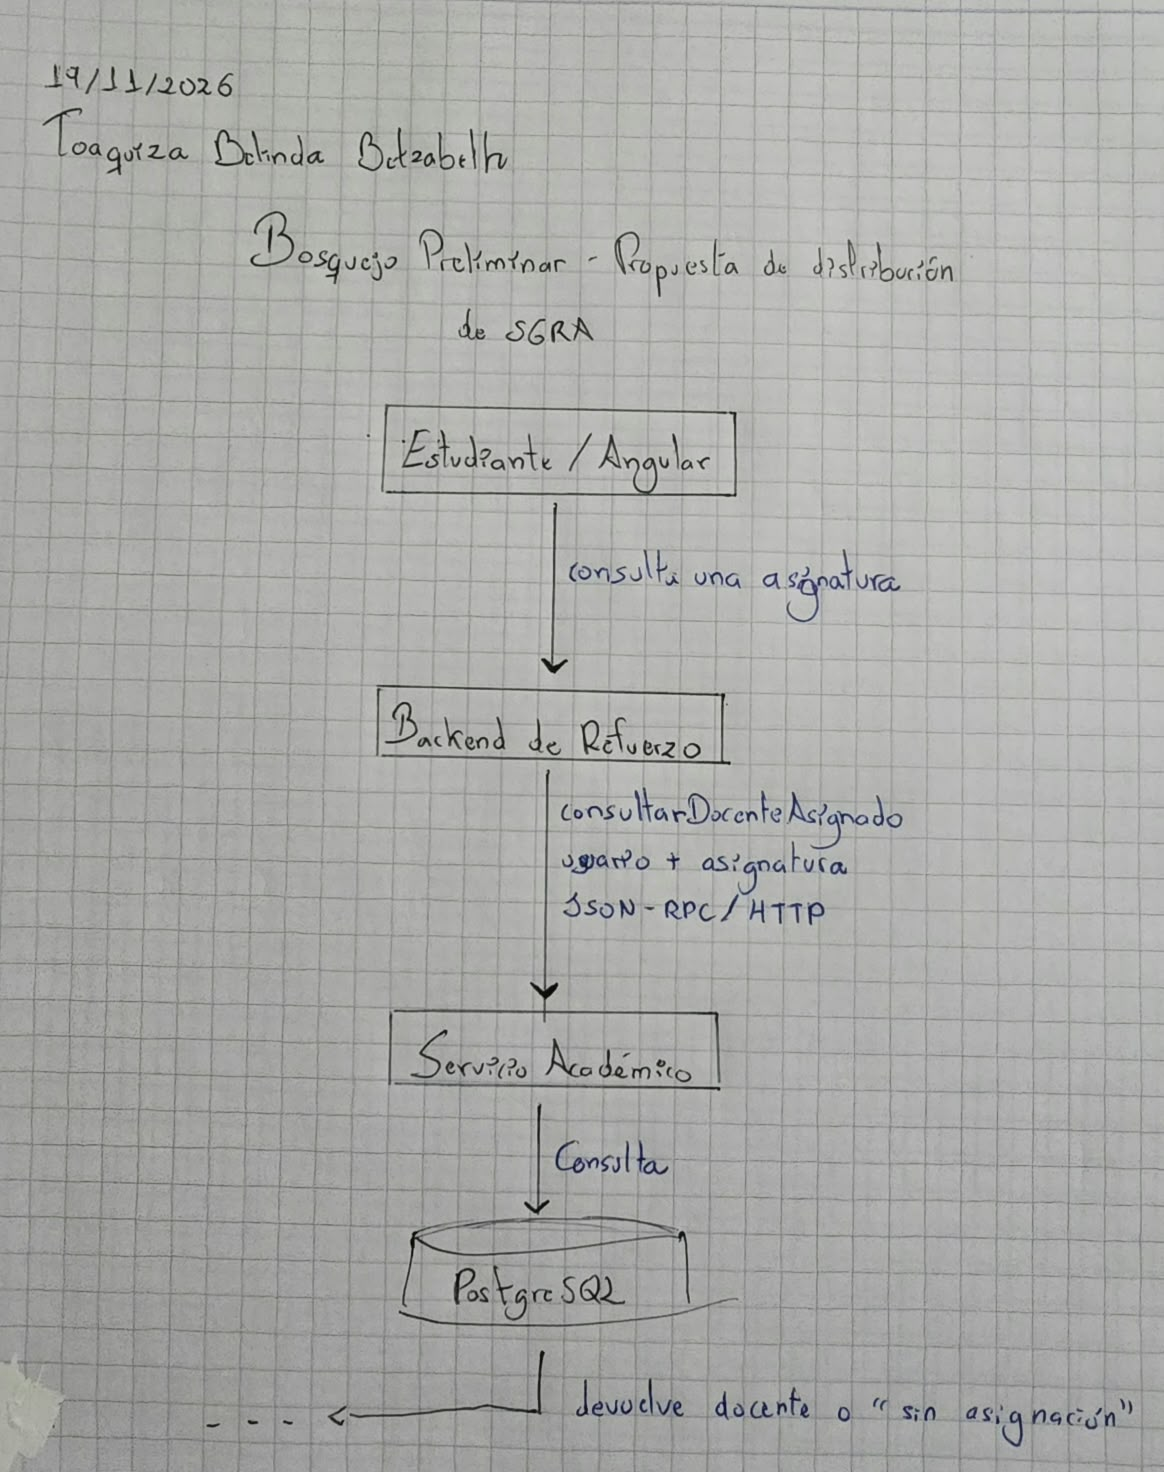
\includegraphics[height=.30\textheight,keepaspectratio]{../evidencias/Belinda T/esquema-mano/sgra-bosquejo-preliminar-consulta-docente-belinda-2026-11-19.jpeg}
\end{center}
{\small Bosquejo original de Belinda Toaquiza, 19 de noviembre de 2026. El diagrama formal precisa los límites de proceso, la identidad autenticada y el retorno de las respuestas. La consulta académica separada es una propuesta futura.}

\newpage
% Notas del integrante 2. Compilar notas/main.tex.
\section*{\personaDos · gRPC}
\small
\textbf{Proyecto}\quad \proyectoDos\par
\subsection*{Teoría y ejemplo sencillo}
gRPC define el servicio en un archivo \texttt{.proto}; de ese contrato se genera el stub del cliente y la base del servidor, y los mensajes viajan en binario con Protocol Buffers sobre HTTP/2 \cite{kaminski2023}. En la demo, \texttt{ClienteTurnos} hace el papel de Inspecciones y llama a \texttt{ConsultarTurno} en \texttt{ServidorTurnos}, que hace el de Turnos y Pagos. Con la placa \texttt{GSA-1234} respondió \texttt{CONFIRMADO}; con \texttt{MBA-0567}, \texttt{PENDIENTE\_PAGO}; con \texttt{XYZ-999}, \texttt{SIN\_TURNO}; y con el servidor apagado el cliente recibió \texttt{UNAVAILABLE} (capturas en \path{evidencias/integrante-2/demo-grpc/}).
\subsection*{Aplicación futura al proyecto}
\textbf{Estado actual.} El prototipo del PFC separa Inspecciones y Turnos y Pagos, cada uno con Spring Boot y su propia base PostgreSQL, y los comunica por REST con \texttt{POST /turnos/\{id\}/autorizaciones-inspeccion}. El equipo midió un p95 de 47,4 ms con 10 usuarios en un equipo local \cite{rtvpfc2026}. \textbf{Supuesto de diseño, no es el estado actual:} llevar esa llamada a gRPC unario y bloqueante con un \emph{deadline} de 3 s, que es el mismo límite que hoy usa REST. Ofrece transparencia de acceso, pero no de fallos. Ante un corte se prioriza la consistencia: sin autorización no se inicia la inspección. Con la red sana también se prioriza la consistencia, porque debe existir una sola autorización por turno. La mejora en latencia no está medida.
\subsection*{Fallo supuesto y conclusión}
Si la autorización se guarda pero la respuesta llega tarde, el cliente recibe \texttt{DEADLINE\_EXCEEDED} aunque el servidor ya escribió \cite{grpcdeadlines}. Por eso el reintento debe llevar la misma clave de idempotencia, como hace Stripe \cite{stripeidempotency}. Antes de cambiar REST por gRPC, implementaría esa clave en el contrato y la validaría demorando el servidor más de 3 s para comprobar que queda una sola autorización.

\begin{minipage}{\linewidth}
\textbf{Anexo: bosquejo a mano}\par\smallskip
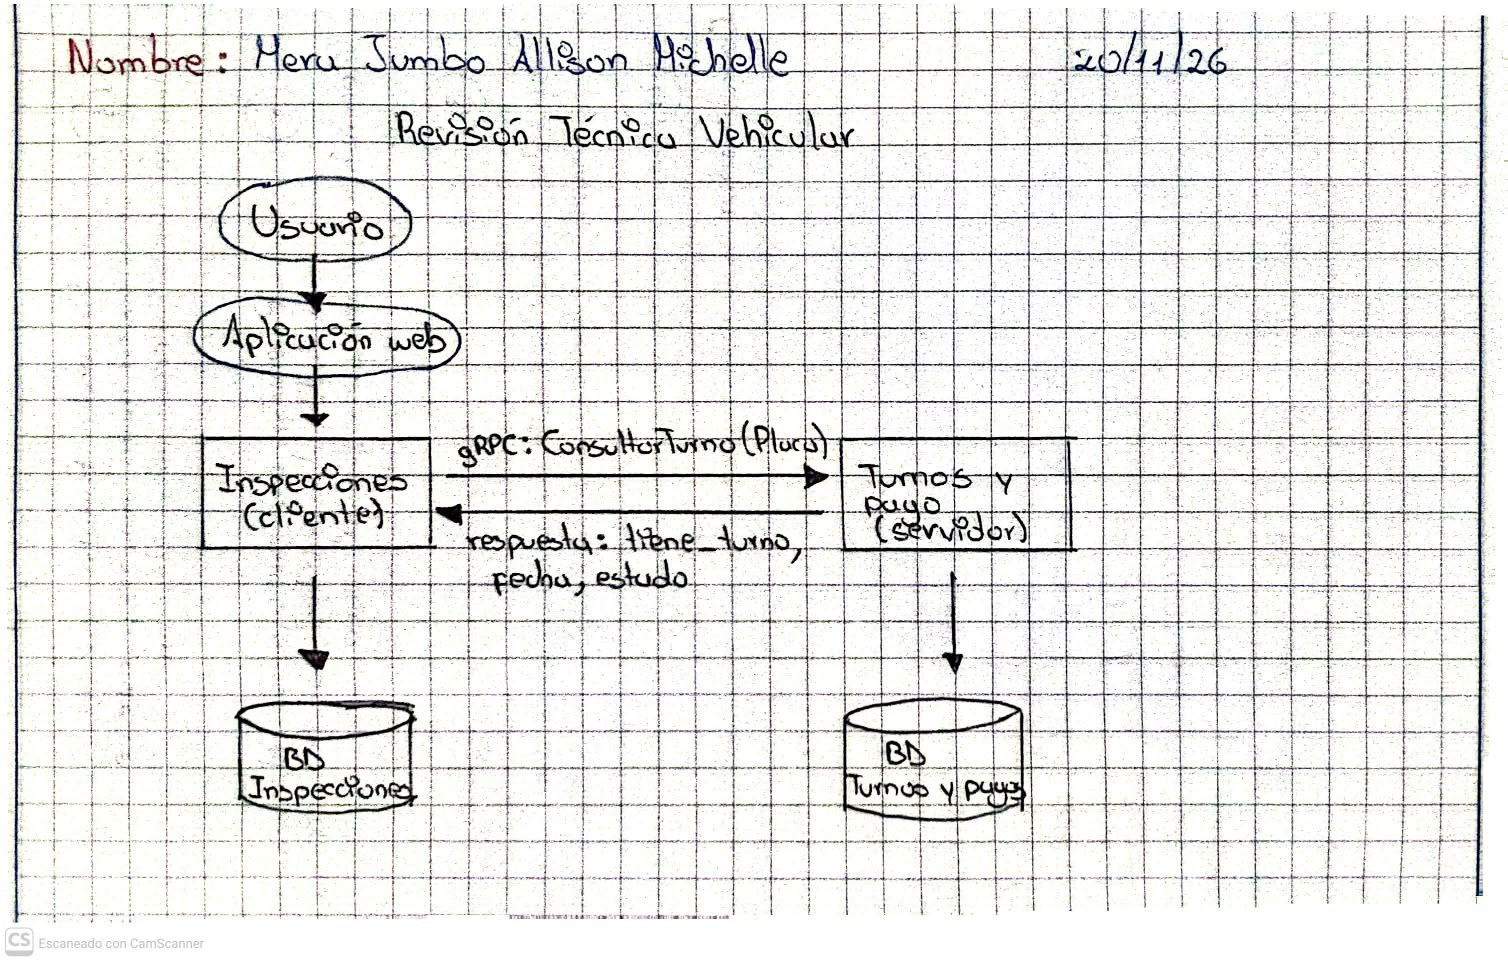
\includegraphics[height=.2\textheight,keepaspectratio]{../evidencias/integrante-2/esquema-mano/esquema-mano-revision-vehicular-grpc-2026-11-20.jpeg}\par
{\footnotesize Bosquejo original de \personaDos, 20 de noviembre de 2026. Vista parcial del RTV: solo la autorización de inicio; la llamada gRPC es supuesta.}
\end{minipage}
\newpage
% Notas del integrante 3. Compilar notas/main.tex.
\section*{\personaTres · Java RMI}
\textbf{Proyecto}\quad \proyectoTres
\subsection*{Teoría y ejemplo sencillo}
\textbf{Turno}\quad Expone \personaTres{} en el tercer turno.\par
Java RMI permite que un programa Java llame a un método de un objeto que vive en otra JVM. El cliente escribe la llamada como si el objeto fuera local. \campo{Citar fuente de esta definición tras leerla.}\par
El ejemplo es un conversor de temperatura en \texttt{demo/integrante-3/}. Tiene tres piezas:
\begin{itemize}
\item \texttt{ConversorRemoto} es el contrato: extiende \texttt{Remote} y declara \texttt{double aFahrenheit(double celsius) throws RemoteException}.
\item \texttt{Servidor} implementa el contrato, exporta el objeto con \texttt{UnicastRemoteObject.exportObject}, crea el registro en el puerto 1099 y lo publica con el nombre \texttt{Conversor}.
\item \texttt{Cliente} busca \texttt{Conversor} en el registro y llama al método.
\end{itemize}
Entrada: 25 C. Salida obtenida en mi ejecución: 77.0 F. El servidor imprimió \texttt{recibi 25.0 C, respondo 77.0 F}, así que la cuenta se hizo en su JVM. El cliente imprimió el tipo \texttt{jdk.proxy1.\$Proxy0}: lo que recibe es un stub, no el objeto real. La captura está en \texttt{evidencias/integrante-3/demo-rmi/01-demo-rmi.png}.
\espacio
\subsection*{Aplicación futura al proyecto}
\textbf{Estado actual del SSDC} (repositorio aldairHub/CHRSweb, commit \texttt{86a238b}). El backend es Java 21 con Spring Boot 4.0.2 (\texttt{backend/pom.xml}); el README indica Spring Boot 3.2 y Java 17, y tomo el \texttt{pom.xml} porque es lo que compila. El código de verificación por correo funciona así:
\begin{itemize}
\item \texttt{VerificacionController}, línea 23: \texttt{/api/verificacion/enviar} llama a \texttt{generarCodigo(correo)} de \texttt{CodigoVerificacionService}, que guarda el código en un \texttt{ConcurrentHashMap} (línea 17) con expiración de 10 minutos (línea 26).
\item Línea 24: el mismo método llama a \texttt{EmailService.enviarCodigoVerificacion}, que guarda el código en un segundo mapa propio (\texttt{EmailService}, líneas 22 y 46) y lo envía por correo.
\item Línea 39: \texttt{/api/verificacion/validar} consulta solo el mapa de \texttt{EmailService} (línea 63). El \texttt{validarCodigo} de \texttt{CodigoVerificacionService} (línea 32), el que revisa la expiración, no tiene ningún llamador.
\end{itemize}
Los dos mapas están en memoria de la JVM del backend. Eso es lo que se lee en el código; no lo he ejecutado.\par
\textbf{Supuesto de diseño, no es el estado actual.} Si el backend corriera en dos instancias, un código generado en una no existiría en la otra. Candidato para exponer con RMI: una interfaz \texttt{VerificacionRemota} con \texttt{generarCodigo(String)} y \texttt{validarCodigo(String, String)}, cuyos argumentos y resultados (\texttt{String} y \texttt{boolean}) son serializables. \campo{Transparencias, CAP/PACELC y comparación con fuentes.}
\espacio
\subsection*{Fallo supuesto y conclusión}
\campo{Describir causa, impacto, detección, recuperación propuesta y prueba de validación.}
\espacio
\textbf{Bosquejo a mano}\quad
\campo{Insertar la foto de evidencias/integrante-3/esquema-mano, con nombres y fecha visibles.}

\newpage
% Notas del integrante 4. Compilar notas/main.tex.
\section*{\personaCuatro · Llamadas y fallos de red}
\textbf{Proyecto}\quad \proyectoCuatro
\subsection*{Teoría y ejemplo sencillo}
\campo{Escribir lo que se dirá sobre Llamadas y fallos de red, el contrato, la entrada y la salida de la demo.}
\espacio
\subsection*{Aplicación futura al proyecto}
\campo{Explicar el estado actual y qué servicio se implementaría. Añadir la operación, motivación, transparencias, CAP/PACELC y comparación con fuentes.}
\espacio
\subsection*{Fallo supuesto y conclusión}
\campo{Describir causa, impacto, detección, recuperación propuesta y prueba de validación.}
\espacio
\textbf{Bosquejo a mano}\quad
\campo{Insertar la foto de evidencias/integrante-4/esquema-mano, con nombres y fecha visibles.}

\section*{Aportes del equipo}
\small
\begin{tabularx}{\linewidth}{lX}
\toprule Integrante & Aporte concreto y evidencia\\\midrule
\personaUno & \campo{Completar}\\
\personaDos & \campo{Completar}\\
\personaTres & \campo{Completar}\\
\personaCuatro & \campo{Completar}\\\bottomrule
\end{tabularx}
\section*{Uso de inteligencia artificial}
Se utilizó inteligencia artificial como apoyo para la búsqueda de fuentes y para formalizar la redacción de las diapositivas y la plantilla. \campo{Completar con los demás usos efectivos.}
\end{document}
